% !TEX root = ../main.tex

%----------------------------------------------------------------------------------------
% ABSTRACT PAGE
%----------------------------------------------------------------------------------------

\begin{abstract}
This work presents an integrated investment framework for energy systems, focusing on 
optimal technology selection and placement of electrical generation, conversion, and storage assets. The core 
engine combines DC Optimal Power Flow (DC-OPF) simulations with linear programming (using the PuLP solver) to 
evaluate both technical feasibility and economic viability across a multi-scenario analysis. A 9-bus test network 
provides the backdrop for a reduced ten distinct cases, each featuring a unique mix of conventional (nuclear, gas) and 
renewable (solar, wind) power plants, supplemented by battery storage of varying capacities.

To balance computational efficiency with seasonal realism, the annual horizon is divided into three representative 
weeks (summer, winter, and spring/autumn), whose costs and operations are subsequently scaled to form a full-year 
analysis. This approach reveals significant seasonal differences in storage utilization even enabling clean assets to
compensate for the cost of conventional generation.

\begin{figure}[H]
    \centering
    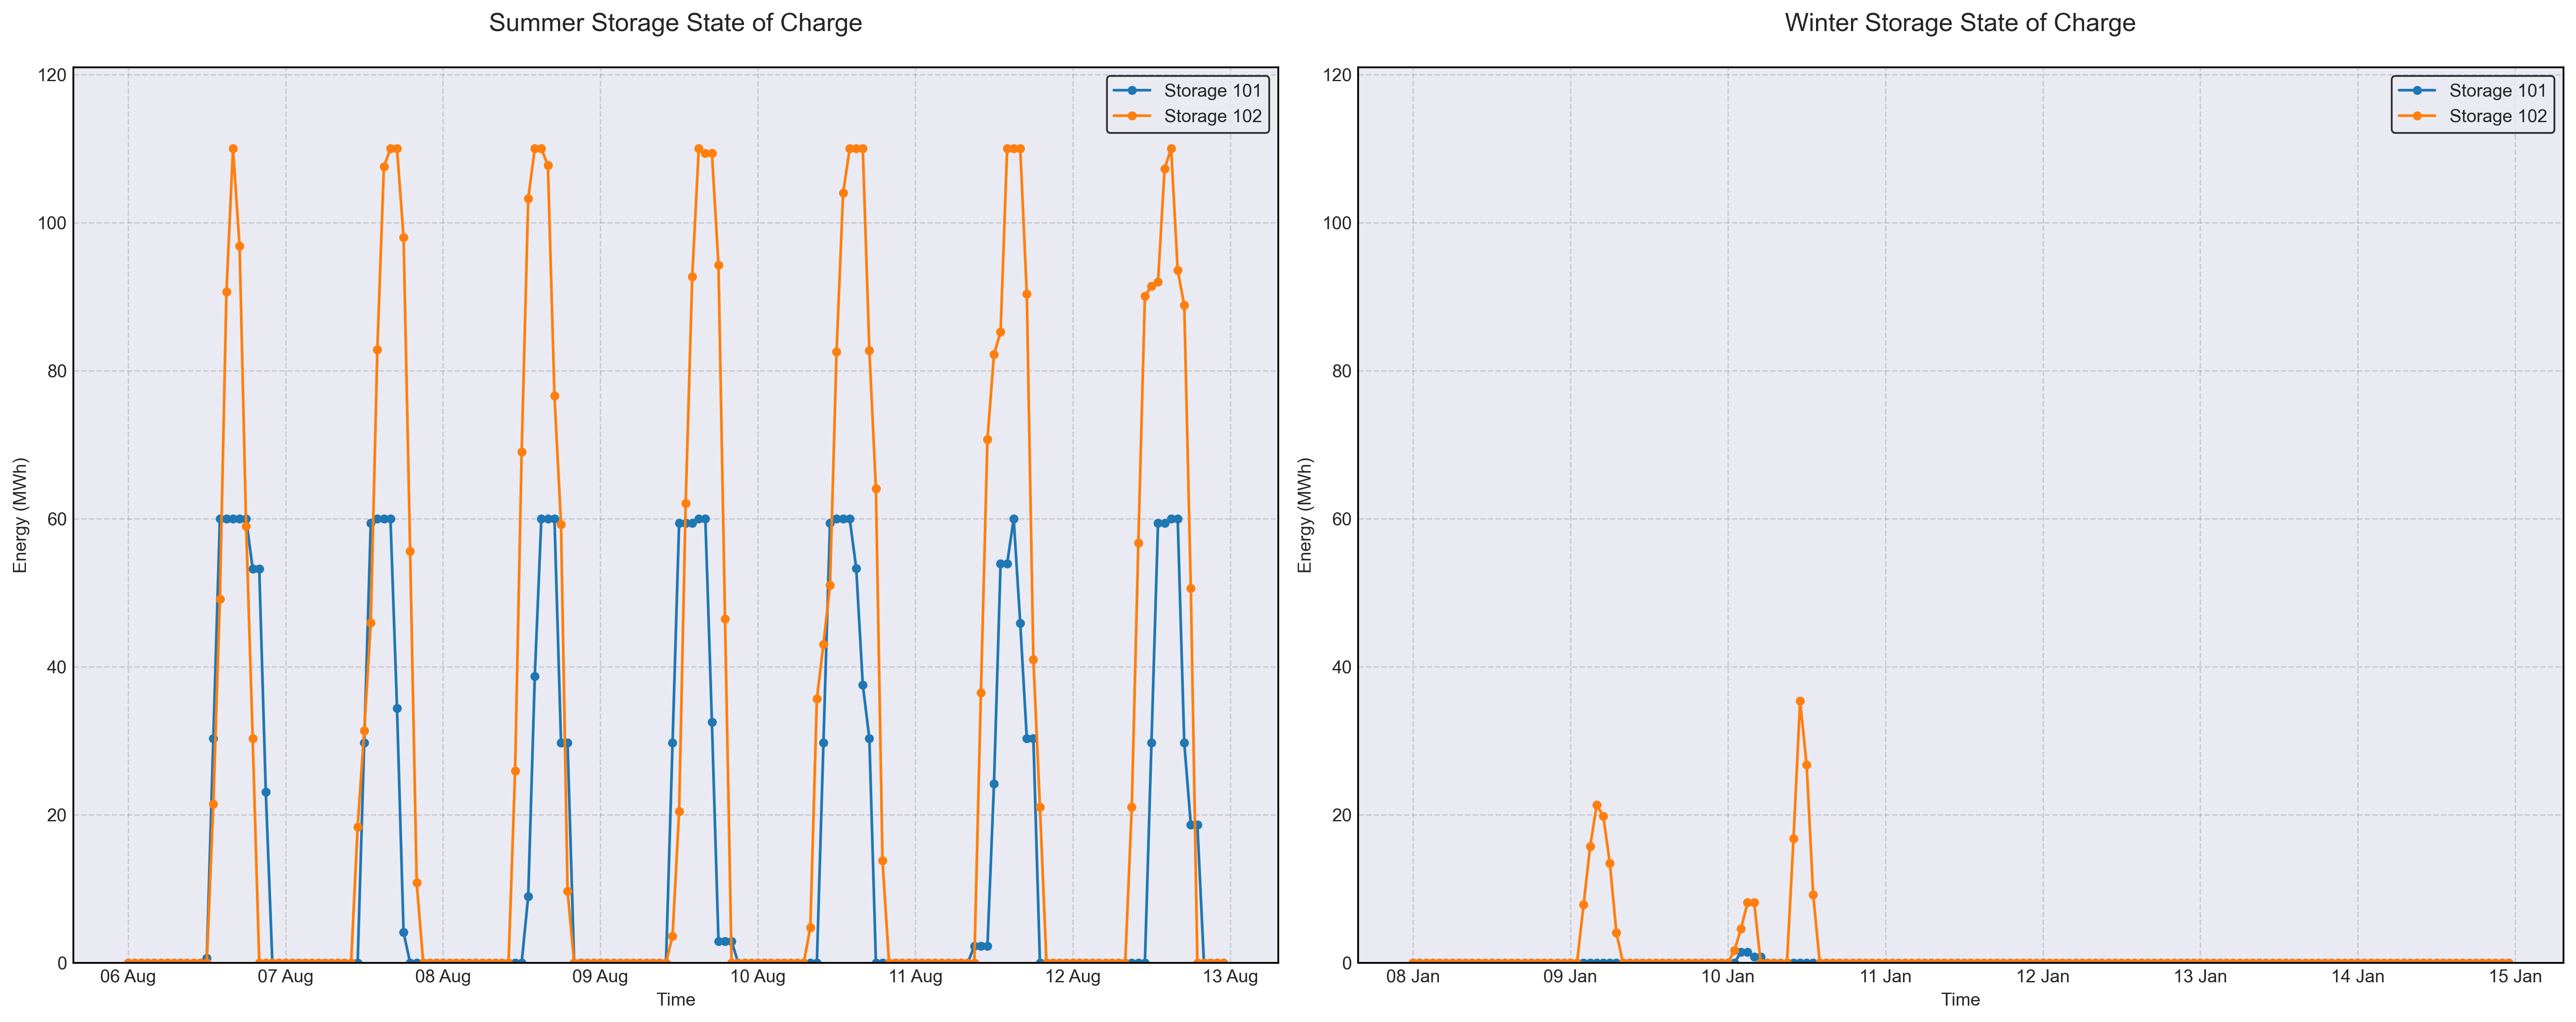
\includegraphics[width=0.6\textwidth]{images/soc_5.png}
    \caption{Summer/Winter battery SoC profile comparison -- Scenario 5}
    \label{fig:soc5}
\end{figure}

In scenarios featuring abundant solar generation, the SoC frequently reaches its upper limits, highlighting the 
potential for upsizing or more flexible operational strategies—such as battery leasing or modular additions—to 
capture peak renewable output.

An economic sensitivity analysis underscores the strong influence of high-cost resources during extreme load 
conditions, causing a disproportionate rise in total costs when reliance on expensive generation escalates. 
Meanwhile, scenarios with nuclear-dominated baseload exhibit lower operational cost volatility but may still 
benefit from targeted storage deployment to manage residual demand swings. AI-assisted reporting consolidates 
these findings by identifying cost drivers, optimal technology mixes, and operational bottlenecks across all 
scenarios. Notably, Scenario7’s balanced blend of nuclear, solar, and wind with moderate battery support emerges 
as the most cost-effective configuration, while Scenario4, featuring gas-fired generation and multiple storage 
units, proves the least favorable in terms of net present value (NPV).

Overall, the proposed framework bridges technical dispatch simulation and investment analysis, guiding stakeholders 
in designing resilient, economically viable energy systems. Future enhancements include broader maintenance modeling, 
real-time price integration for advanced arbitrage strategies, and further prompt-engineering improvements to refine 
AI-driven reporting and decision support.

\textbf{Keywords:} \keywordnames

%DC-OPF, Investment Analysis, Linear Programming, Renewable Integration, 
%Power Systems Planning, Asset Placement Optimization
\end{abstract}
\newpage